\documentclass[xcolor=dvipsnames]{beamer}

\usetheme{Boadilla}

\newcommand{\bi}{\begin{itemize}}
\newcommand{\ei}{\end{itemize}}
\newcommand{\be}{\begin{enumerate}}
\newcommand{\ee}{\end{enumerate}}
\newcommand{\I}{\item}
\newcommand{\f}{\frame}
\newcommand{\ft}{\frametitle}


\begin{document}

\title{Least-Squares Fitter Summary}
\author[M.\ Ito]{Mark M.\ Ito}
\date{March 5, 2009}
\institute[JLab]{Jefferson Lab}

\f{
\ft{Least-Squares Track Fitter}
\bi
\I Uses Levenberg-Marquardt algorithm from GNU Scientific Library (from MINPACK)
\I Not a finder
\I Initial parameters estimated from hit list
\I Swim particles through magnetic field
\I Works with FDC hits, CDC hits, or any combination
\I CDC: time residuals, FDC: pseudopoint space residual
\I Constant errors, CDC: $150~\mu$m, FDC: $200~\mu$m
\I Track parameters:
  \be
  \I Total inverse momentum: $1/p_t$
  \I Polar angle: $\theta$
  \I Azimuthal angle: $\phi$
  \I Transverse distance of point of closest approach to beamline: $r_0$
  \I Z of point of closest approach to beamline: $z_0$
  \ee
\ei
}

\f{
\ft{Five parameters, fitted - true}
$$
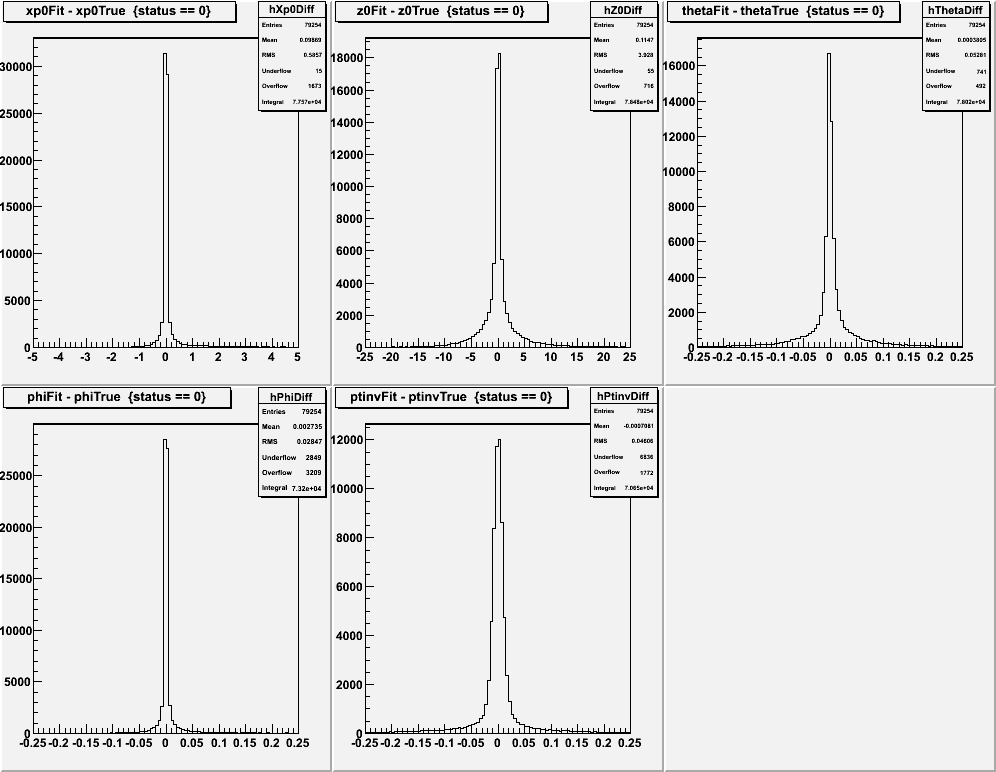
\includegraphics[height=3.0in]{standard74.png}
$$
}

\f{
\ft{fit efficiency, total momentum vs. polar angle}
$$
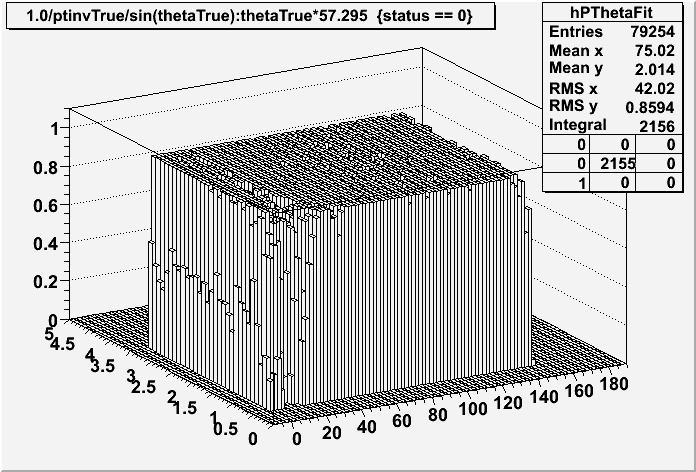
\includegraphics[height=3.0in]{standard11.png}
$$
}

\f{
\ft{Iterations, $\chi^2$, and $\chi^2$ probability}
$$
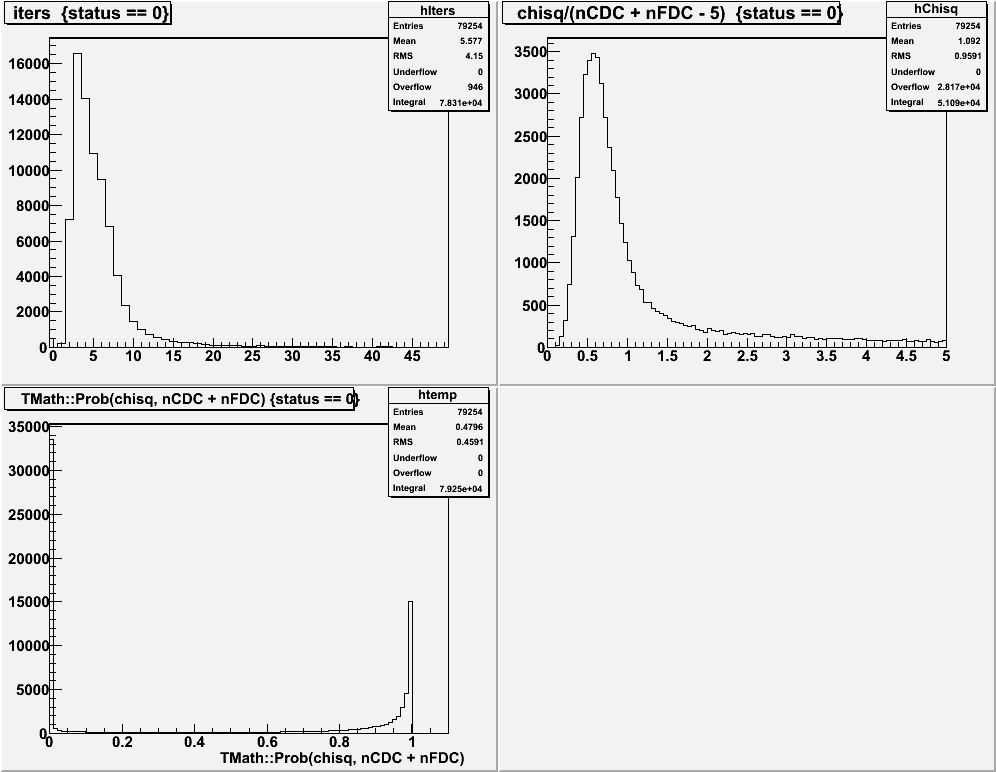
\includegraphics[height=3.0in]{standard84.png}
$$
}

\f{
\ft{Issues}
\be
\I Non-converging events: few percent
\I What is the source of anomalous probability distribution?
  \be
  \I FDC? CDC? Both?
  \I Particular regions of phase space?
  \I Out-of-time hits in ``pure'' (background free) one track events?
  \ee
\I FDC errors
  \be
  \I anode drift time and each cathode should be separate measurements
  \I error from cathode should be a function of ionization
  \I error from anode should reflect smearing of drift time
  \ee
\I Need to look at true vs.\ fitted chisq ``parameter chi-squared''
$$
\chi^2 = R^T C^{-1} R
$$

where $R$ is a vector of residuals: $r_i = x_{i,{\rm measured}} - x_{i,{\rm true}}$, $i$ runs over the five parameters and $C$ is the covariance
matrix of the fit.
  \be
  \I Which parameter(s) is (are) out-of-line?
  \I What are the correlations among parameters?
  \ee
\ee
}

\end{document}

%%% end of latex file %%%%
